\section{Using the supply side: costs, conduct and counterfactuals}\label{sec:04-supply}

\Cref{sec:04-bertrand,sec:04-diversion,sec:04-existence} characterized the pricing equilibrium and the conditions
under which it exists and is unique. We now put the pricing rule to work. The first-order conditions
\eqref{eq:04-foc-matrix} tie together four objects: the demand system and its
derivatives, the ownership matrix, prices and marginal costs. Given any three of them, the conditions restrict
the fourth. This section uses them in three directions. With estimated demand, observed prices and an assumed
ownership structure, they recover marginal costs without any cost data (\cref{sec:04-mc}). With demand and
independent information on margins, they let us compare models of conduct (\cref{sec:04-conduct}). With
demand, recovered costs and a changed environment, they predict the new equilibrium
(\cref{sec:04-counterfactuals,sec:04-comparative}). We begin with the reasons for modeling supply at all.

\subsection{Why model supply when we estimate demand?}\label{sec:04-supply-why}

Write the markup equation \eqref{eq:04-markup} product by product, and let marginal cost depend on observed
\emph{cost shifters} $w_j$ (variables that move cost but not utility) and an unobserved cost shock $\omega_j$:
\begin{equation}\label{eq:04-price-decomp}
p_j = mc_j(w_j, \omega_j) + m_j(p, x, \xi;\, \theta_d, \Omega),
\qquad m = -\big(\Omega \odot \Delta^\top\big)^{-1} q .
\end{equation}
Here $\theta_d$ collects the demand parameters, $x$ and $\xi$ stack the observed and unobserved characteristics
of all products, and $m_j$ is the $j$th element of the markup vector $m$. Equation \eqref{eq:04-price-decomp} is
a model of price. A product's price moves with its own cost and with every determinant of its markup, including
the characteristics and prices of all other products. Three reasons to model supply follow from it.

\casehead{Prices are endogenous, and supply tells us which instruments are valid}
Take the logit demand of \cref{sec:04-bertrand-logit}, with mean utility $\delta_j = x_j\beta - \alpha p_j +
\xi_j$. Firms observe the unobserved quality $\xi_j$ when they set prices, so $p_j$ responds to it. For a
single-product firm the pricing condition is $p_j = mc_j + \frac{1}{\alpha(1 - s_j)}$ by
\cref{prop:04-logit-markup}. Hold rivals' prices fixed and define
\begin{equation*}
F(p_j, \xi_j) \equiv p_j - mc_j - \frac{1}{\alpha(1 - s_j)} = 0 .
\end{equation*}
The logit derivatives \eqref{eq:04-logit-derivs} give $\frac{\partial s_j}{\partial p_j} = -\alpha s_j(1 - s_j)$,
and the same algebra gives $\frac{\partial s_j}{\partial \xi_j} = s_j(1 - s_j)$. Differentiating $F$,
\begin{align*}
\frac{\partial F}{\partial p_j} &= 1 - \frac{1}{\alpha(1 - s_j)^2}\,\frac{\partial s_j}{\partial p_j}
  = 1 + \frac{s_j}{1 - s_j} = \frac{1}{1 - s_j}, \\
\frac{\partial F}{\partial \xi_j} &= -\frac{1}{\alpha(1 - s_j)^2}\,\frac{\partial s_j}{\partial \xi_j}
  = -\frac{s_j}{\alpha(1 - s_j)} .
\end{align*}
By the implicit function theorem (\cref{app:math}),
\begin{equation}\label{eq:04-dp-dxi}
\frac{d p_j}{d \xi_j} = -\frac{\frac{\partial F}{\partial \xi_j}}{\frac{\partial F}{\partial p_j}}
= \frac{s_j}{\alpha(1 - s_j)}\,(1 - s_j) = \frac{s_j}{\alpha} > 0 .
\end{equation}
Products with high unobserved quality carry high prices. In the logit estimating equation $\ln s_j - \ln s_0 =
x_j\beta - \alpha p_j + \xi_j$ of \cref{ch:logit}, the regressor $p_j$ is therefore positively correlated with the
error $\xi_j$. Least squares biases the price coefficient $-\alpha$ toward zero, and estimated demand looks too
inelastic.

The price equation also tells us which variables can serve as instruments. A valid instrument moves $p_j$ and is
uncorrelated with $\xi_j$. By \eqref{eq:04-price-decomp} three groups of variables move prices. Cost shifters
$w_j$ move $mc_j$ and are excluded from utility. Characteristics of other products move $m_j$ through shares and
diversion ratios, and they are excluded from the utility of product $j$. Changes in ownership move $m_j$ through
$\Omega$. \citet[eq.~(4.1)]{BerryLevinsohnPakes1995} state the identifying assumption as $\E[\xi_j \mid z] =
\E[\omega_j \mid z] = 0$, where $z$ stacks the characteristics and cost shifters of all products.
\Cref{ch:logit,ch:blp} develop these instruments, and \cref{sec:06-charinst} explains why instruments built from
characteristics fail when firms choose characteristics with knowledge of $\xi_j$.

\casehead{The pricing equation adds information about demand}
Suppose we specify $mc_j = w_j\gamma + \omega_j$ and fix $\Omega$. For any candidate value of $\theta_d$ we can
compute the markups $m(\theta_d)$ at observed prices and quantities, and with them the implied cost shock
\begin{equation*}
\omega_j(\theta_d, \gamma) = p_j - m_j(\theta_d) - w_j\gamma .
\end{equation*}
Moment conditions $\E[z_j\,\omega_j(\theta_d, \gamma)] = 0$ then restrict $\theta_d$ as well as $\gamma$. A price
coefficient that is too small in absolute value, for example, implies markups that are too large. The implied
costs are then too low exactly where markups are high, and they become correlated with instruments that shift
markups. \citet{BerryLevinsohnPakes1995} estimate demand and the pricing equation jointly for this reason
(\cref{ch:blp}).

\casehead{Markups, costs and counterfactuals require a model of price setting}
Demand alone yields elasticities and diversion ratios. Markups require a model of how prices are set, and so do
the marginal costs inferred from them. Every counterfactual that changes prices, such as a merger, a new product
or a tax, requires solving for a new equilibrium.

These reasons come with a trade-off. Demand can usually be estimated without specifying supply in full.
Instruments motivated by supply, such as cost shifters, remain valid whatever the exact model of conduct, as long
as they are excluded from utility and uncorrelated with $\xi_j$. Adding the pricing equation brings more
information and more assumptions. If conduct or the cost function is misspecified, joint estimation transmits the
error into the demand estimates. The researcher therefore trades efficiency against robustness. Counterfactuals
need a model of supply in any case, so the assumptions return at that stage even when estimation avoids them.

\subsection{Recovering marginal costs}\label{sec:04-mc}

Suppose demand has been estimated, with parameter estimate $\hat\theta_d$, and that we observe prices $p$ and
quantities $q$ in a market. The demand Jacobian $\Delta(p; \hat\theta_d)$ can then be evaluated at the observed
prices. We rearrange \eqref{eq:04-foc-matrix} in two steps:
\begin{align*}
\big(\Omega \odot \Delta^\top\big)(p - mc) &= -q, \\
p - mc &= -\big(\Omega \odot \Delta^\top\big)^{-1} q .
\end{align*}
Solving for marginal cost gives the \emph{implied} (or recovered) marginal cost
\begin{equation}\label{eq:04-mc-recover}
\widehat{mc} = p + \big(\Omega \odot \Delta(p; \hat\theta_d)^\top\big)^{-1} q .
\end{equation}
\Cref{prop:04-markup-positive} guarantees that the inverse exists and that the implied markups are positive
whenever some of every product's lost sales go to the outside good. With market size $M$, $q = Ms$ and
$\Delta = M\Delta^s$, so the same formula holds with shares and share derivatives. The computation is done market
by market, and it uses no cost data.

\begin{remark}[What cost recovery assumes]\label{rem:04-mc-assumptions}
Formula \eqref{eq:04-mc-recover} rests on four assumptions. (i) The demand model is correctly specified and
$\hat\theta_d$ is consistent. (ii) Observed prices satisfy the first-order conditions of a static
simultaneous-move pricing game, with interior prices. (iii) The matrix $\Omega$ describes conduct correctly.
(iv) Marginal cost is constant, or the recovered value is read as marginal cost at the observed output. The
formula does not require the equilibrium to be unique. \citet[fn.~12]{BerryLevinsohnPakes1995} note that ``none
of the properties of the estimates require uniqueness of equilibrium.'' Uniqueness matters only at the
counterfactual stage (\cref{sec:04-counterfactuals}).
\end{remark}

With logit demand the inversion has a closed form. By \cref{prop:04-logit-markup} every product of firm $f$
carries the markup $\frac{1}{\alpha(1 - S_f)}$, where $S_f$ is the firm's combined share. Hence
\begin{equation}\label{eq:04-mc-logit}
\widehat{mc}_j = p_j - \frac{1}{\hat\alpha\,\big(1 - S_{f(j)}\big)} .
\end{equation}
Within a firm, differences in recovered costs equal differences in prices. Across firms, a product of a firm with
a larger combined share is assigned a larger markup, and so a lower cost at a given price.

\begin{example}[Cost recovery under three models of conduct]\label{ex:04-mc-recovery}
Treat the multi-product equilibrium (M) of \cref{ex:04-logit25} as data. Its prices range from 0.744 to 1.852,
and the true marginal costs range from 0.164 to 1.236. We apply \eqref{eq:04-mc-recover} with the true $\alpha
= 2$ and three ownership matrices.
\begin{enumerate}
  \item With the true owners, the recovered costs equal the true costs up to rounding error.
  \item If we wrongly assume single-product firms ($\Omega = I_{25}$), the implied markups are
  $\frac{1}{\alpha(1 - s_j)}$, between 0.502 and 0.568. The recovered costs then exceed the true costs by 0.014 to
  0.168, by 0.098 on average, against a mean true cost of 0.767.
  \item If we assume that one owner sets all 25 prices ($\Omega = \mathbf{1}\mathbf{1}^\top$), every markup equals
  $\frac{1}{\alpha s_0} = \frac{1}{2 \times 0.1601} = 3.12$. All 25 recovered costs are negative, with mean $-1.74$.
\end{enumerate}
Assuming too little internalization overstates costs, and assuming too much understates them. The third case
shows that implausible implied costs can reject a model of conduct outright.
\end{example}

\casehead{Why the New Empirical IO avoids accounting costs}
Formula \eqref{eq:04-mc-recover} is the answer of the New Empirical Industrial Organization to the unreliability
of accounting cost data \citep{Bresnahan1989}, discussed in \cref{ch:intro,ch:conduct}. Accounting data have
four problems for our purpose. First, they report average (variable) cost, which differs from marginal cost
unless returns to scale are constant. Second, multi-product firms share plants, distribution and advertising, and
accountants allocate these common costs across products by conventions without economic content. Third,
accounting depreciation follows tax and reporting rules, and the opportunity cost of capital and of owned inputs
is missing \citep{FisherMcGowan1983}. Fourth, the data are reported by firm or division, not by product and
market. The structural approach trades these measurement problems for dependence on the demand model and on the
assumed conduct. Accounting data then become a check on the model. \citet[p.~333]{Nevo2001}, for example, uses
accounting margins only as a crude benchmark. He treats Census margins, built from average variable costs, as an
upper bound on price-cost margins.

\casehead{The cost equation}
We often want to know what determines the recovered costs: input prices, returns to scale, the cost of
characteristics, or the savings from a merger. The standard specification projects marginal cost on cost
shifters:
\begin{equation}\label{eq:04-cost-eq}
mc_j = w_j\gamma + \omega_j
\qquad\text{or}\qquad
\ln mc_j = w_j\gamma + \omega_j ,
\end{equation}
where $w_j$ is a row vector of observed cost shifters and $\omega_j$ is the unobserved cost shock.
\citet[eq.~(3.1)]{BerryLevinsohnPakes1995} use the log form. Their $w_j$ contains product characteristics, and they
note that $\omega_j$ may be correlated with $\xi_j$ because larger cars, or cars with higher unobserved quality,
may cost more to produce (p.~853).

\citet{BerryLevinsohnPakes1995} write the first-order conditions with the opposite sign convention. Their $J
\times J$ matrix has element $(j, r)$ equal to $-\frac{\partial s_r}{\partial p_j}$ when products $r$ and $j$ have
the same owner and zero otherwise (their eq.~3.4). In our notation it is $-(\Omega \odot \Delta^{s\top})$. Their
first-order conditions read $s - \Delta^{\mathrm{BLP}}(p - mc) = 0$, and their markup is
\begin{equation}\label{eq:04-blp-markup}
b(p, x, \xi; \theta) = \big(\Delta^{\mathrm{BLP}}\big)^{-1}s = -\big(\Omega \odot \Delta^{s\top}\big)^{-1}s
\end{equation}
(their eq.~3.5). Substituting into \eqref{eq:04-cost-eq} gives the \emph{pricing equation} that is taken to the
data,
\begin{equation}\label{eq:04-cost-est}
p_j - b_j(\hat\theta_d) = w_j\gamma + \omega_j
\qquad\text{or}\qquad
\ln\big(p_j - b_j(\hat\theta_d)\big) = w_j\gamma + \omega_j ,
\end{equation}
where the log version is their eq.~(3.6). The left side is the recovered marginal cost $\widehat{mc}_j$.

\casehead{Why the error enters additively}
Because $\omega_j$ enters \eqref{eq:04-cost-est} additively, we can solve for it at any parameter value:
$\omega_j(\theta_d, \gamma) = \widehat{mc}_j(\theta_d) - w_j\gamma$. Given instruments $z_j$, the moment
conditions
\begin{equation}\label{eq:04-supply-moment}
\E\big[z_j^\top\,\omega_j(\theta_{d0}, \gamma_0)\big] = 0
\end{equation}
are linear in $\gamma$ for fixed $\theta_d$, so $\gamma$ is estimated by linear instrumental variables. If the
cost shock entered nonseparably, for example as $mc_j = c(w_j, \omega_j)$ with $c$ not invertible in $\omega_j$,
we could not compute the residual and these moments would be unavailable. Additivity is what makes the
econometrics simple.

\casehead{When the cost equation needs instruments}
With $\theta_d$ known and constant marginal cost, \eqref{eq:04-cost-est} is a regression of cost on its
determinants, and least squares is consistent if $\E[\omega_j \mid w_j] = 0$. Three features of applications
break this condition. First, $w_j$ often includes output, as in $\ln mc_j = w_j\gamma + \gamma_q\ln q_j + \omega_j$,
to allow for returns to scale. A high $\omega_j$ raises $p_j$ and lowers $q_j$, so $q_j$ is correlated with the
error. Second, the characteristics in $w_j$ may have been chosen with knowledge of $\omega_j$. Third, tests of
conduct place the markup on the right side with a free coefficient $\vartheta$, as in $p_j = w_j\gamma +
\vartheta\, b_j + \omega_j$. Here \citet[p.~854]{BerryLevinsohnPakes1995} point out that ``since $p$ is a function of $\omega$,
$b(p, x, \xi; \theta)$ is a function of $\omega$'' and cannot be assumed uncorrelated with it. In each case we
need excluded instruments, such as demand shifters and characteristics of rival products, which move output or
markups but are mean independent of $\omega_j$.

\casehead{The recovered cost is a generated regressand}
The left side of \eqref{eq:04-cost-est} depends on $\hat\theta_d$. Consistency of $\hat\gamma$ follows from
consistency of $\hat\theta_d$. The usual standard errors are wrong, however, because they ignore the estimation
error in $\hat\theta_d$. With least squares on the stacked cost shifters $\mathcal{W}$, a first-order expansion gives
\begin{equation}\label{eq:04-generated}
\hat\gamma - \gamma_0 \approx \big(\mathcal{W}^\top \mathcal{W}\big)^{-1}\mathcal{W}^\top\Big[\omega + \frac{\partial\,\widehat{mc}(\theta_{d0})}
{\partial\theta_d^\top}\big(\hat\theta_d - \theta_{d0}\big)\Big].
\end{equation}
The second term adds variance, and it is correlated across all products and markets that share $\hat\theta_d$.
There are two remedies. We can stack the demand and supply moments into one GMM problem and use its joint
asymptotic variance (\cref{ch:blp,app:econometrics}). Or we can bootstrap, resampling markets and re-estimating
demand in each replication.

\begin{example}[Cost regressions under three models of conduct]\label{ex:04-cost-regression}
Continue \cref{ex:04-mc-recovery}. The true costs satisfy $mc_j = x_j\gamma + \omega_j$ with $\gamma = (0.2,
0.25, 0.3)$, where $x_j$ contains a constant, a continuous characteristic and a binary characteristic. A least
squares regression of the true costs on $x_j$ gives $\hat\gamma = (0.182, 0.250, 0.310)$, with standard errors
$(0.025, 0.010, 0.020)$. Costs recovered with the true owners give the same estimates. Costs recovered under
single-product conduct give $(0.303, 0.239, 0.305)$. Costs recovered under one owner give $(-2.301, 0.235, 0.316)$.
The conduct error loads almost entirely on the intercept here, because logit markups vary little with the
characteristics. In richer demand models markup errors are correlated with characteristics, and they bias the
slopes too.
\end{example}

\subsection{Conduct and the ownership matrix}\label{sec:04-conduct}

Bertrand-Nash pricing with the true owners is one model of conduct. We now embed it in a family of models
indexed by profit weights. This makes conduct comparable with the conduct parameter $\theta$ of
\cref{ch:conduct}.

\begin{definition}[Profit weights and the generalized ownership matrix]\label{def:04-profit-weights}
Let $\kappa_{fg} \ge 0$ be the weight that firm $f$ places on the profit of firm $g$, with $\kappa_{ff} = 1$.
Firm $f$ chooses the prices of its products to maximize
\begin{equation}\label{eq:04-kappa-objective}
\pi_f + \sum_{g \neq f}\kappa_{fg}\,\pi_g ,
\end{equation}
taking the prices of other firms as given. The \emph{generalized ownership matrix} $\Omega(\kappa)$ has elements
$\Omega(\kappa)_{jk} = \kappa_{f(j)f(k)}$, where $f(j)$ is the owner of product $j$.
\end{definition}

The symbol $\kappa$ denotes profit weights throughout this chapter. \Cref{ch:conduct} uses the same letter for a
different object.

\begin{lemma}[First-order conditions with profit weights]\label{lem:04-kappa-foc}
With profit weights $\kappa$, the first-order conditions of all firms are
\begin{equation}\label{eq:04-foc-kappa}
q + \big(\Omega(\kappa) \odot \Delta^\top\big)(p - mc) = 0 .
\end{equation}
\end{lemma}

\begin{proof}
Firm $g$'s profit is $\pi_g = \sum_{k \in \mathcal{J}_g}(p_k - mc_k)q_k(p)$ with constant marginal costs. Take
$j \in \mathcal{J}_f$ and differentiate \eqref{eq:04-kappa-objective} with respect to $p_j$. The own-profit term
gives $q_j + \sum_{k \in \mathcal{J}_f}(p_k - mc_k)\frac{\partial q_k}{\partial p_j}$, as in
\eqref{eq:04-foc-scalar}. The term for firm $g \neq f$ gives $\kappa_{fg}\sum_{k \in \mathcal{J}_g}(p_k -
mc_k)\frac{\partial q_k}{\partial p_j}$, because $p_j$ enters $\pi_g$ only through the quantities. Adding the terms
and using $\kappa_{ff} = 1$,
\begin{equation*}
q_j + \sum_{k = 1}^{J}\kappa_{f(j)f(k)}\,(p_k - mc_k)\frac{\partial q_k}{\partial p_j} = 0 .
\end{equation*}
The coefficient of $(p_k - mc_k)$ is $\Omega(\kappa)_{jk}\Delta_{kj} = (\Omega(\kappa) \odot \Delta^\top)_{jk}$, so
stacking over $j$ gives \eqref{eq:04-foc-kappa}.
\end{proof}

Row $j$ of $\Omega(\kappa)$ describes the objective of the firm that sets $p_j$. The matrix need not be
symmetric, because $\kappa_{fg}$ and $\kappa_{gf}$ can differ. Cost recovery \eqref{eq:04-mc-recover},
counterfactuals and pass-through all go through with $\Omega(\kappa)$ in place of $\Omega$. Four cases are
standard.
\begin{enumerate}
  \item \emph{Nash pricing} sets $\kappa_{fg} = 0$ for $f \neq g$, so $\Omega(\kappa) = \Omega$.
  \item \emph{Full collusion}, or joint profit maximization, sets $\kappa_{fg} = 1$ for all $f$ and $g$, so
  $\Omega(\kappa) = \mathbf{1}\mathbf{1}^\top$. Whether such conduct can be sustained is the subject of
  \cref{ch:collusion-theory}.
  \item A \emph{merger} of firms $f$ and $g$ sets $\kappa_{fg} = \kappa_{gf} = 1$ and leaves the other weights at
  zero.
  \item \emph{Partial internalization} has weights strictly between zero and one. Joint ventures and moderate
  common ownership produce such weights.
\end{enumerate}
These cases span the range $\kappa_{fg} \in [0, 1]$, from Nash pricing to joint profit maximization. Many conduct
models restrict the weights to this range. The restriction is an additional assumption, and the common-ownership
weights below need not satisfy it.

\casehead{Common ownership}
\citet{OBrienSalop2000} derive profit weights from ownership stakes. Let investors $h = 1, \dots, H$ hold
cash-flow shares $\lambda_{gh}$ in firm $g$, and let $\eta_{fh}$ be investor $h$'s share of control over firm
$f$. (The symbols $\lambda$, $\eta$, $h$ and $H$ are local to this paragraph.) Suppose the manager of firm $f$
maximizes the control-weighted sum of its investors' portfolio profits:
\begin{equation*}
\sum_{h = 1}^{H}\eta_{fh}\sum_{g = 1}^{F}\lambda_{gh}\,\pi_g
= \sum_{g = 1}^{F}\Big(\sum_{h = 1}^{H}\eta_{fh}\lambda_{gh}\Big)\pi_g .
\end{equation*}
Dividing by the coefficient on $\pi_f$ leaves the maximizer unchanged and gives the form
\eqref{eq:04-kappa-objective} with
\begin{equation}\label{eq:04-obrien-salop}
\kappa_{fg} = \frac{\sum_{h}\eta_{fh}\lambda_{gh}}{\sum_{h}\eta_{fh}\lambda_{fh}} ,
\end{equation}
provided that the investors who control $f$ hold some cash-flow stake in $f$, so that the denominator is positive.
The weight is large when the investors who control $f$ own large cash-flow stakes in $g$. Nothing bounds it by
one. If the sole controlling investor of $f$ holds 10 percent of $f$ and 90 percent of $g$, then
$\kappa_{fg} = \frac{0.9}{0.1} = 9$. The manager of $f$ then values a dollar of $g$'s profit at nine dollars of
its own.
\citet{BackusConlonSinkinson2021} compute such weights for the ready-to-eat cereal industry and ask whether
pricing reflects them.

\casehead{Joint ventures}
\citet{MillerWeinberg2017} study the 2008 joint venture that combined the US operations of SABMiller and Molson
Coors. The Department of Justice approved the transaction on June 5, 2008, on the ground that efficiencies in
brewing would outweigh any adverse competitive effect \citep[p.~241, n.~161]{AskerNocke2021}. Almost immediately after
clearance, the prices of 12-packs of Miller Lite, Bud Light and Coors Light rose by about 8 percent. The imported
flagship brands Corona Extra and Heineken show little persistent change \citep[p.~242]{AskerNocke2021}. Miller and
Weinberg's demand system is a random coefficients nested logit. On the supply side, a weight $\kappa \in [0, 1]$ captures coordination between
brands that are not jointly owned. It enters the ownership matrix of the standard first-order conditions and is
estimated. A weight of zero is Nash pricing, and a weight of one is joint profit maximization. The estimate rejects
unilateral price competition \citep[p.~242, n.~164]{AskerNocke2021}. In their specification the weight applies to
pairs of products of Anheuser-Busch InBev (ABI) and MillerCoors in the periods after the joint venture
\citep[Section~5.1, p.~1779]{MillerWeinberg2017}. \Cref{ch:mergers} treats the application.

\begin{remark}[Profit weights and the conduct parameter]\label{rem:04-kappa-theta}
Profit weights give the conduct parameter of \cref{ch:conduct} a structural reading. Let $N$ symmetric Cournot
firms with constant marginal cost $c$ each maximize $\pi_i + \kappa\sum_{l \neq i}\pi_l$, with $\pi_l = (P(Q) -
c)q_l$. The first-order condition of firm $i$ is
\begin{equation*}
P(Q) - c + P'(Q)\Big(q_i + \kappa\sum_{l \neq i}q_l\Big) = 0 .
\end{equation*}
At a symmetric equilibrium $q_i = \frac{Q}{N}$, so $q_i + \kappa\sum_{l \neq i}q_l = \frac{1 + \kappa(N - 1)}{N}Q$
and
\begin{equation*}
P(Q) = c - \frac{1 + \kappa(N - 1)}{N}\,Q\,P'(Q) .
\end{equation*}
This is the supply relation \eqref{eq:03-supply-relation} with $\theta = \frac{1 + \kappa(N - 1)}{N}$. Nash
behavior ($\kappa = 0$) gives the Cournot value $\theta = \frac{1}{N}$, and full collusion ($\kappa = 1$) gives
$\theta = 1$. With differentiated products, however, conduct is a matrix. We therefore compare a short menu of
ownership matrices, or estimate a low-dimensional $\kappa$, rather than a free parameter for every pair of
products.
\end{remark}

\casehead{Testing conduct}
Two ownership matrices $\Omega^A$ and $\Omega^B$ imply two markup vectors and two vectors of recovered costs. There
are four main ways to choose between them. First, implied costs may be implausible, as the negative costs of
\cref{ex:04-mc-recovery} are. Second, implied margins can be compared with independent measures of margins, as in
\citet{Nevo2001} below. Third, nonnested tests compare the fit of the full models, as in the 1955 automobile
price war studied by \citet{Bresnahan1987} (\cref{sec:06-bresnahan}). A \emph{nonnested test} compares two models,
neither of which is a special case of the other. Fourth, under the true model the implied
cost shock is mean independent of excluded instruments, while under a false model it generally is not.
\citet[Section~6, p.~1776]{BerryHaile2014} give a formal foundation, in a much more general setting, to the
intuition of \citet{Bresnahan1982}, discussed in \cref{sec:03-rotation}. Their results allow product differentiation and do not require rotations of
demand. Variation in the number of competing firms, the set of competing goods, or the characteristics or costs of
competitors can discriminate between models of conduct (p.~1779).

\casehead{An application: margins in ready-to-eat cereal}
\citet{Nevo2001} estimates a random coefficients demand system for 25 brands of ready-to-eat cereal and uses the
pricing equation to decompose margins (\cref{ch:blp} gives the full case study). His supply side writes the
first-order conditions as $s(p) - \Omega(p - mc) = 0$, where $\Omega_{jr} = \Omega^*_{jr}S_{jr}$, $S_{jr} =
-\frac{\partial s_r}{\partial p_j}$, and $\Omega^*$ is the ownership matrix. This is the convention of
\citet{BerryLevinsohnPakes1995}. The implied markups are (his eq.~1, p.~313)
\begin{equation}\label{eq:04-nevo-markup}
p - mc = \Omega^{-1}s(p) .
\end{equation}
Nevo evaluates \eqref{eq:04-nevo-markup} under three structures. With \emph{single-product firms}, each brand is
priced by an agent who cares only about that brand, and margins reflect product differentiation alone. With the
\emph{current ownership} of the brands by multi-product firms, margins also reflect the internalization of
substitution among a firm's brands. With \emph{joint ownership} of all brands, margins are those of a monopolist
or of a perfect cartel. The margins of the three structures define a decomposition,
\begin{equation}\label{eq:04-nevo-decomp}
m^{\mathrm{joint}} = \underbrace{m^{\mathrm{single}}}_{\text{differentiation}}
+ \underbrace{\big(m^{\mathrm{current}} - m^{\mathrm{single}}\big)}_{\text{portfolio effect}}
+ \underbrace{\big(m^{\mathrm{joint}} - m^{\mathrm{current}}\big)}_{\text{collusion effect}} .
\end{equation}
Each term is nonnegative product by product when goods are substitutes (\cref{prop:08-nevo-ownership}).

The three structures imply very different margins. With the full random coefficients model, the median margin $\frac{p - mc}{p}$ over
27,862 brand-city-quarter observations is 35.8 percent with single-product firms. It is 42.2 percent under current
ownership and 72.6 percent under joint ownership of the 25 brands \citep[Table~VIII]{Nevo2001}. Product
differentiation thus accounts for most of the predicted margin, and the portfolio effect adds 6.4 percentage
points. Joint profit maximization would add 30.4 points more. Nevo compares these predictions with a gross retail
margin of 46.0 percent from accounting sources. The price gap between national brands and private labels gives a
lower bound of about 31 percent (p.~333). He rejects joint profit maximization of the 25 brands, whose 95
percent confidence interval runs from 62.2 to 97.2 percent. He cannot reject multi-product Nash pricing, whose
interval runs from 29.1 to 55.8 percent (p.~334).

The logit version of the same exercise illustrates why the demand model matters for conduct. With logit demand,
the median margins are 33.6, 35.8 and 41.9 percent under the three structures, and 54.0 percent if all brands in
the market are priced jointly \citep[Table~VIII]{Nevo2001}. The mean price sensitivity of the full model is close
to the logit price coefficient. The gap between the models widens from single-product to joint ownership, because
the full model captures cross-price substitution better (p.~332). By \cref{prop:04-logit-markup}, logit markups
depend on ownership only through combined shares. When those shares are small, as they are when the outside good is
large, internalizing rival brands changes logit margins little.
Nevo notes that with the logit estimates one cannot reject full collusion over all products, and he attributes
this to the strong assumptions of the logit rather than to conduct (p.~335). A demand model that hardly
distinguishes conduct structures cannot test them. \Cref{tab:08-nevo-margins} in \cref{ch:blp} reproduces the full
table.

\subsection{Counterfactual analysis}\label{sec:04-counterfactuals}

A counterfactual asks what would happen under conditions never observed: a merger that has not occurred, a
product not yet launched, a tax not yet levied. Answering it requires a model whose primitives remain valid under
the new conditions.

\begin{definition}[Structural model and counterfactual]\label{def:04-structural}
A model is \emph{structural} with respect to a change in the environment if its primitives do not change when the
environment changes. Here the primitives are the demand parameters and unobserved qualities $\xi$, the cost
function and cost shocks $\omega$, and the rule of conduct. A
\emph{counterfactual} is the equilibrium of the model after one element of the environment is changed, with all
other primitives held at their estimated values.
\end{definition}

\begin{remark}[The counterfactual algorithm]\label{rem:04-algorithms}
A static counterfactual in a differentiated-products market proceeds in five steps.
\begin{enumerate}
  \item \emph{Estimate demand} from data on the status quo, with instruments for price (\cref{ch:logit,ch:blp}).
  Recover $\hat\xi$ along with $\hat\theta_d$.
  \item \emph{Recover marginal costs} at the observed prices and quantities from \eqref{eq:04-mc-recover}, using
  the status quo ownership matrix $\Omega^0$. Optionally estimate the cost equation \eqref{eq:04-cost-eq} and
  recover $\hat\omega$.
  \item \emph{Change the environment.} A merger, a divestiture or collusion changes the ownership matrix to
  $\Omega^1$ (for instance by setting to one the entries for pairs of products of the merging firms). Entry, exit or
  a new good changes the product set (\cref{ch:newgoods}). A new product needs characteristics $x_{J+1}$, an assumed
  quality $\xi_{J+1}$ (often zero, the mean of $\xi$) and a marginal cost from the cost equation. A tax, a tariff, an
  input-price change or a merger efficiency changes marginal costs: $mc_j + t_j$ for a specific tax $t_j$, and
  $(1 - E_j)mc_j$ for a proportional efficiency $E_j$, as in \eqref{eq:04-upp}.
  \item \emph{Solve for the new equilibrium}, that is, find $p^1$ with
  \begin{equation*}
  q(p^1) + \big(\Omega^1 \odot \Delta(p^1)^\top\big)\big(p^1 - mc^1\big) = 0 ,
  \end{equation*}
  using the demand model to evaluate $q(\cdot)$ and $\Delta(\cdot)$ at every trial price vector.
  \item \emph{Compute outcomes}, namely price and share changes, firms' profits, and consumer surplus from the
  demand model. With logit demand and market size $M$, the change in consumer surplus is $\frac{M}{\alpha}\ln\frac{\Phi^1}
  {\Phi^0}$, where $\Phi = 1 + \sum_k e^{\delta_k}$ (\cref{ch:logit}). With random coefficients the log-sum is
  integrated over consumers, each term divided by that consumer's $\alpha_i$.
\end{enumerate}
\end{remark}

Step 4 is the computational core. Four solution methods are common.
\begin{enumerate}
  \item \emph{Best-response iteration.} Each firm in turn maximizes its profit given the others' current prices,
  and the process repeats until prices stop changing. It converges when the best-response map is a contraction, as
  in the single-product logit (\cref{prop:04-logit-br}). With logit demand each step has the Lambert-W closed form
  of \cref{sec:04-bertrand-logit}.
  \item \emph{Markup iteration.} Iterate $p \leftarrow mc - (\Omega \odot \Delta(p)^\top)^{-1}q(p)$. The update is
  simple, but nothing guarantees convergence. Damped updates, which move prices only part of the way toward the
  right side, often help.
  \item \emph{Newton's method.} Write the stacked conditions as $G(p) = q(p) + (\Omega \odot \Delta(p)^\top)(p -
  mc)$ and iterate $p \leftarrow p - [\frac{\partial G}{\partial p^\top}]^{-1}G(p)$. Convergence is quadratic near
  the solution. The Jacobian involves second derivatives of demand, given in \eqref{eq:04-dGdp} below, and the
  method can wander when it starts far from the solution.
  \item \emph{The Morrow-Skerlos iteration.} For random coefficients logit demand with price coefficient $\alpha_i > 0$,
  split the share Jacobian as $\Delta^s(p) = -\Lambda(p) + \Gamma(p)$, with the diagonal matrix
  $\Lambda_{jj}(p) = \int\alpha_i s_{ij}(p)\,\dd F$ and the symmetric matrix $\Gamma_{jk}(p) = \int\alpha_i
  s_{ij}(p)s_{ik}(p)\,\dd F$. Here $s_{ij}$ is consumer $i$'s choice probability. The first-order conditions are
  then equivalent to the fixed point \citep{MorrowSkerlos2011}
  \begin{equation}\label{eq:04-ms}
  p - mc = \zeta(p) \equiv \Lambda(p)^{-1}\Big[s(p) + \big(\Omega \odot \Gamma(p)\big)(p - mc)\Big],
  \end{equation}
  which is iterated as $p \leftarrow mc + \zeta(p)$. The derivation is \cref{prop:08-ms} in \cref{ch:blp}. In the
  plain logit, $\Lambda = \alpha\diag(s)$ and $\Gamma = \alpha ss^\top$, so \eqref{eq:04-ms} becomes $m_j =
  \frac{1}{\alpha} + \sum_k\Omega_{jk}s_k m_k$. This is the fixed point of \cref{prop:04-logit-markup}.
\end{enumerate}

Whatever the method, convergence must be checked. We stop when the sup-norm change in prices falls below a tight
tolerance, such as $10^{-12}$, and then verify the first-order conditions directly. A residual in price units,
such as $\|\zeta(p) - (p - mc)\|_\infty$, is more informative than a residual in share units, which becomes small
at very high prices where every share is small. First-order conditions do not guarantee that each firm is at a
global maximum. Where profit may have several local maxima in own price (\cref{ex:04-multiple-eq}), we also
evaluate each firm's profit over a grid of unilateral deviations.

\casehead{Equilibrium selection}
\Cref{sec:04-multiple} showed that a counterfactual can have several equilibria even when estimation is
unaffected. An iterative solver selects the equilibrium in whose basin of attraction it starts, so the common
practice of starting from the status quo prices is itself a selection rule. A careful analysis restarts the solver
from many points and reports every equilibrium it finds. With logit demand and constant marginal costs the issue
does not arise, because the equilibrium is unique for every ownership structure (\cref{thm:04-logit-unique}).

\begin{example}[A simulated merger]\label{ex:04-merger-sim}
In the 25-product market of \cref{ex:04-logit25}, take the multi-product equilibrium (M) as the status quo and let
owners 3 and 4 merge. They hold 6 and 7 products with combined shares of 21.40 and 25.36 percent. We hold
marginal costs fixed and solve for the post-merger equilibrium with all four methods, starting from the
pre-merger prices. Best-response iteration and the Morrow-Skerlos iteration converge in 17 steps, markup iteration
needs 91 steps, and Newton's method with the analytic Jacobian \eqref{eq:04-dGdp} converges in 6 iterations. All
four reach the same prices, within
$5 \times 10^{-14}$. Five hundred random starting points lead to the same equilibrium, as
\cref{thm:04-logit-unique} implies. \Cref{tab:04-merger-sim} reports the results.
\end{example}

\begin{table}[htbp]
\centering
\caption{A simulated merger of owners 3 and 4 in the 25-product logit market}
\label{tab:04-merger-sim}
\footnotesize
\begin{tabular}{@{}lcccccccc@{}}
\toprule
 & & \multicolumn{2}{c}{Combined share (\%)} & \multicolumn{2}{c}{Markup} & Price & \multicolumn{2}{c}{Profit $\times 100$} \\
\cmidrule(lr){3-4}\cmidrule(lr){5-6}\cmidrule(l){8-9}
Owner & Products & Pre & Post & Pre & Post & change & Pre & Post \\
\midrule
\multicolumn{9}{@{}l}{\textit{Panel A. Owners}} \\
0 & 3 & 18.87 & 21.23 & 0.616 & 0.635 & 0.018 & 11.632 & 13.476 \\
1 & 3 & 4.67 & 5.41 & 0.524 & 0.529 & 0.004 & 2.449 & 2.857 \\
2 & 6 & 13.68 & 15.56 & 0.579 & 0.592 & 0.013 & 7.925 & 9.214 \\
3 (merging) & 6 & 21.40 & 17.25 & 0.636 & 0.821 & 0.185 & 13.616 & 14.167 \\
4 (merging) & 7 & 25.36 & 21.87 & 0.670 & 0.821 & 0.151 & 16.989 & 17.959 \\
\midrule
\multicolumn{9}{@{}l}{\textit{Panel B. Market}} \\
\multicolumn{3}{@{}l}{Outside share $s_0$} & 0.1601 & 0.1869 & & & & \\
\multicolumn{3}{@{}l}{Consumer surplus $\frac{1}{\alpha}\ln\Phi$} & 0.9159 & 0.8387 & & & & \\
\multicolumn{3}{@{}l}{Total profit} & 0.5261 & 0.5767 & & & & \\
\multicolumn{3}{@{}l}{Total surplus} & 1.4421 & 1.4154 & & & & \\
\multicolumn{3}{@{}l}{Share-weighted mean price} & 1.3553 & 1.4465 & & & & \\
\bottomrule
\end{tabular}

\vspace{3pt}
\begin{minipage}{0.97\textwidth}
\footnotesize Notes: Pre is the multi-product equilibrium (M) of \cref{tab:04-logit25}. Post is the equilibrium
after owners 3 and 4 merge, with marginal costs unchanged. Every product of an owner has the same markup and so
the same price change. Market size is one. Computed with \texttt{figures/ch04/src/supply\_examples.py}.
\end{minipage}
\end{table}

The merged firm prices all 13 of its products at the common markup 0.821. This equals $\frac{1}{\alpha(1 -
S)}$ at its post-merger combined share $S = 0.3912$, as \cref{prop:04-logit-markup} requires. The prices of
former owner 3 rise by 0.185 and those of former owner 4 by 0.151. Most of the increase is the merged firm's
unilateral response. If the merged firm best-responds to the unchanged pre-merger prices of its rivals, its markup
is 0.817. Rivals' price increases, between 0.004 and 0.018, add only 0.004 to it through strategic
complementarity.

The outsiders gain more than the merging parties. The merging parties' combined profit rises from 30.605 to
32.126 (times 100), while the rivals' combined profit rises from 22.006 to 25.547. The merged firm restricts its
own sales to raise price, and the rivals capture the diverted customers at higher prices. This free-riding
reappears in merger theory (\cref{ch:mergers}). Consumer surplus falls by 8.4 percent, the outside share rises
from 16.0 to 18.7 percent, and total surplus falls by 0.027.

How large would merger efficiencies need to be to leave consumers unharmed? With logit demand the answer has a
closed form. All prices stay at their pre-merger levels if and only if the merged firm's first-order condition
holds at the pre-merger prices. At those prices shares are unchanged, so the merged firm's markup must equal
$\frac{1}{\alpha(1 - S_3 - S_4)} = \frac{1}{2(1 - 0.4676)} = 0.939$. Marginal costs must therefore fall by $0.939
- 0.636 = 0.303$ for the products of owner 3 and by $0.939 - 0.670 = 0.269$ for those of owner 4. Re-solving the
equilibrium with these costs returns the pre-merger prices exactly. Such compensating cost reductions
\citep{Werden1996} are large here: 46 percent of owner 3's average marginal cost and 37 percent of owner 4's.

\subsection{Comparative statics and pass-through}\label{sec:04-comparative}

How do equilibrium prices respond to small changes in costs? The answer gives pass-through of taxes and input
prices, and it converts pricing pressure from a merger into price changes. We derive the general formula and then
evaluate it for logit demand.

\casehead{The general formula}
Write the stacked first-order conditions as a function of prices and marginal costs,
\begin{equation}\label{eq:04-G}
G(p; c) \equiv q(p) + \big(\Omega \odot \Delta(p)^\top\big)(p - c) = 0 ,
\end{equation}
with $c$ the vector of constant marginal costs. Row $j$ reads $G_j = q_j + \sum_k\Omega_{jk}\frac{\partial
q_k}{\partial p_j}(p_k - c_k)$. Differentiating with respect to $c_l$ gives
\begin{equation*}
\frac{\partial G_j}{\partial c_l} = -\Omega_{jl}\frac{\partial q_l}{\partial p_j},
\qquad\text{so}\qquad
\frac{\partial G}{\partial c^\top} = -\big(\Omega \odot \Delta^\top\big).
\end{equation*}
Differentiating with respect to $p_l$ gives three terms, one from $q_j$, one from the markup of product $l$, and
one from the dependence of the derivatives on prices:
\begin{equation*}
\frac{\partial G_j}{\partial p_l} = \frac{\partial q_j}{\partial p_l} + \Omega_{jl}\frac{\partial q_l}{\partial p_j}
+ \sum_k \Omega_{jk}(p_k - c_k)\frac{\partial^2 q_k}{\partial p_j\,\partial p_l} .
\end{equation*}
In matrix form,
\begin{equation}\label{eq:04-dGdp}
\frac{\partial G}{\partial p^\top} = \Delta + \Omega \odot \Delta^\top + H,
\qquad H_{jl} = \sum_k\Omega_{jk}\,m_k\,\frac{\partial^2 q_k}{\partial p_j\,\partial p_l} .
\end{equation}
If $\frac{\partial G}{\partial p^\top}$ is nonsingular at the equilibrium, the implicit function theorem
(\cref{app:math}) shows that equilibrium prices are locally a differentiable function of costs, with
\begin{equation}\label{eq:04-passthrough-matrix}
\frac{\partial p}{\partial c^\top} = -\Big[\frac{\partial G}{\partial p^\top}\Big]^{-1}\frac{\partial G}{\partial c^\top}
= \big[\Delta + \Omega \odot \Delta^\top + H\big]^{-1}\big(\Omega \odot \Delta^\top\big).
\end{equation}
For a single-product monopolist the matrices are scalars, and \eqref{eq:04-passthrough-matrix} reduces to
$\frac{q'}{2q' + (p - c)q''}$. This is the monopoly pass-through formula \eqref{eq:02-pt-monopoly} of
\cref{ch:theory}. The second derivatives in $H$ show that pass-through depends on the curvature of demand as
well as on its slope. A specific tax $t_j$ enters exactly like a cost, so \eqref{eq:04-passthrough-matrix} also gives
tax pass-through. The same formula holds with $\Omega(\kappa)$ in place of $\Omega$.

\casehead{Partial and full pass-through}
It helps to separate a firm's own response from the feedback through rivals' prices. For single-product firms,
let $BR_j(p_{-j}; c_j)$ be firm $j$'s best response, assumed differentiable. Define the \emph{partial pass-through}
$\rho^{\mathrm{p}}_j = \frac{\partial BR_j}{\partial c_j}$, which holds rivals' prices fixed, and the matrix $R$ of
best-response slopes, with $R_{jk} = \frac{\partial BR_j}{\partial p_k}$ for $k \neq j$ and $R_{jj} = 0$.

\begin{lemma}[Equilibrium pass-through from best responses]\label{lem:04-br-passthrough}
If $I - R$ is nonsingular at the equilibrium, then
\begin{equation}\label{eq:04-br-passthrough}
\frac{\partial p}{\partial c^\top} = (I - R)^{-1}\diag\big(\rho^{\mathrm{p}}\big).
\end{equation}
If moreover $\rho^{\mathrm{p}} > 0$, $R \geq 0$ element by element and every row sum of $R$ is below one, then
every element of $(I - R)^{-1} - I$ is nonnegative. Equilibrium own pass-through then weakly exceeds partial pass-through,
and a cost increase for one firm weakly raises every rival's price.
\end{lemma}

\begin{proof}
In equilibrium $p_j = BR_j(p_{-j}; c_j)$ for every $j$. Totally differentiating,
\begin{equation*}
dp_j = \sum_{k \neq j}R_{jk}\,dp_k + \rho^{\mathrm{p}}_j\,dc_j ,
\qquad\text{so}\qquad
(I - R)\,dp = \diag\big(\rho^{\mathrm{p}}\big)\,dc .
\end{equation*}
Multiplying by $(I - R)^{-1}$ gives \eqref{eq:04-br-passthrough}. If $R \geq 0$ with row sums below one, then
$\|R\|_\infty < 1$, so the Neumann series $(I - R)^{-1} = \sum_{n \geq 0}R^n$ converges. Every term is
nonnegative, so $(I - R)^{-1} - I = \sum_{n \geq 1}R^n \geq 0$. Since $\rho^{\mathrm{p}}_j > 0$, the diagonal of
$\frac{\partial p}{\partial c^\top}$ is at least $\rho^{\mathrm{p}}_j$ and the off-diagonal elements are nonnegative.
\end{proof}

\begin{proposition}[Partial pass-through with logit demand]\label{prop:04-passthrough}
Let demand be logit with constant marginal costs, and hold the prices of all other firms fixed.
\begin{enumerate}[label=(\roman*)]
  \item A single-product firm passes through the fraction $\frac{\partial p_j}{\partial c_j} = 1 - s_j$ of a cost
  increase.
  \item If the cost of product $j$ of a multi-product firm $f$ rises, then $\frac{\partial p_j}{\partial c_j} = 1 -
  s_j$, and the price of every other product $l \in \mathcal{J}_f$ falls, with $\frac{\partial p_l}{\partial c_j}
  = -s_j$.
  \item If the costs of all products of firm $f$ rise by the same amount $dc$, every price of firm $f$ rises by
  $(1 - S_f)\,dc$.
\end{enumerate}
\end{proposition}

\begin{proof}
By \cref{prop:04-logit-markup}, whatever its costs, firm $f$'s optimal prices satisfy $p_l = c_l + m_f$ for all
$l \in \mathcal{J}_f$, with a common markup that solves
\begin{equation}\label{eq:04-logit-foc-firm}
\alpha\, m_f\,(1 - S_f) = 1 .
\end{equation}
The firm's best response is the unique solution of this condition (\cref{sec:04-bertrand-logit}). After a change
in costs, the price changes are therefore $dp_l = dc_l + dm_f$.

First we compute how $S_f$ responds. By \eqref{eq:04-logit-derivs}, for $l \in \mathcal{J}_f$,
\begin{equation*}
\frac{\partial S_f}{\partial p_l} = \sum_{k \in \mathcal{J}_f}\frac{\partial s_k}{\partial p_l}
= -\alpha s_l(1 - s_l) + \sum_{k \in \mathcal{J}_f, k \neq l}\alpha s_k s_l = -\alpha s_l(1 - S_f).
\end{equation*}
Hence
\begin{equation*}
dS_f = -\alpha(1 - S_f)\sum_{l \in \mathcal{J}_f}s_l\,dp_l
= -\alpha(1 - S_f)\Big[\sum_{l \in \mathcal{J}_f}s_l\,dc_l + S_f\,dm_f\Big].
\end{equation*}
Next we differentiate \eqref{eq:04-logit-foc-firm}: $(1 - S_f)\,dm_f = m_f\,dS_f$. Substituting $dS_f$ and
$\alpha m_f = \frac{1}{1 - S_f}$ from \eqref{eq:04-logit-foc-firm},
\begin{align*}
(1 - S_f)\,dm_f &= -\alpha m_f(1 - S_f)\Big[\sum_{l}s_l\,dc_l + S_f\,dm_f\Big]
                 = -\Big[\sum_{l}s_l\,dc_l + S_f\,dm_f\Big], \\
dm_f &= -\sum_{l \in \mathcal{J}_f}s_l\,dc_l .
\end{align*}
The markup falls by the share-weighted cost increase. For part (ii), only $dc_j \neq 0$, so $dm_f = -s_j\,dc_j$.
Then $dp_j = (1 - s_j)\,dc_j$ and $dp_l = -s_j\,dc_j$ for $l \neq j$. Part (i) is part (ii) with
$\mathcal{J}_f = \{j\}$. For part (iii), $dc_l = dc$ for all $l \in \mathcal{J}_f$, so $dm_f = -S_f\,dc$ and
$dp_l = (1 - S_f)\,dc$.
\end{proof}

Part (i) is the residual-demand result of \cref{ex:02-pt-examples} in \cref{ch:theory}. Logit residual demand is
log-concave, so pass-through is below one (\cref{cor:02-bulow-pfleiderer}). Part (ii) is less familiar. A cost
increase on one product lowers the firm's combined share, and with it the firm's market power. The firm's common
markup falls, so it cuts the prices of its other products. Part (iii) shows that a multi-product firm with a large
combined share absorbs a large fraction of firm-wide cost shocks.

\begin{corollary}[Equilibrium pass-through with single-product logit firms]\label{cor:04-passthrough-eq}
With single-product logit firms and constant marginal costs,
\begin{equation}\label{eq:04-logit-pt-eq}
\frac{\partial p}{\partial c^\top} = (I - R)^{-1}\diag(1 - s),
\qquad R_{jk} = \frac{s_j s_k}{1 - s_j}\ (k \neq j).
\end{equation}
Own equilibrium pass-through exceeds $1 - s_j$, and every rival's price rises. In a symmetric market with $J$
products of share $s$ each and outside share $s_0 = 1 - Js > 0$, an industry-wide cost increase is passed through
at the rate $\frac{(1 - s)^2}{1 - s - (J - 1)s^2} < 1$.
\end{corollary}

\begin{proof}
The slopes $R_{jk} = \frac{s_j s_k}{1 - s_j}$ are the logit best-response slopes of \cref{prop:04-logit-br}, and
$\rho^{\mathrm{p}}_j = 1 - s_j$ by \cref{prop:04-passthrough}. Formula \eqref{eq:04-br-passthrough} gives
\eqref{eq:04-logit-pt-eq}. Let $S = \sum_k s_k = 1 - s_0 < 1$. Row $j$ of $R$ sums to
\begin{equation*}
\sum_{k \neq j}\frac{s_j s_k}{1 - s_j} = \frac{s_j(S - s_j)}{1 - s_j} < \frac{s_j(1 - s_j)}{1 - s_j} = s_j < 1,
\end{equation*}
so \cref{lem:04-br-passthrough} applies. In the symmetric case every off-diagonal element of $R$ equals $\bar R =
\frac{s^2}{1 - s}$, so every row of $R$ sums to $(J - 1)\bar R$. With an equal cost increase for all products the
equilibrium is symmetric, $dp = \bar\rho\,dc\,\mathbf{1}$ for a scalar $\bar\rho$, and $(I - R)\,dp = (1 -
s)\,dc\,\mathbf{1}$ gives
\begin{equation*}
\bar\rho = \frac{1 - s}{1 - (J - 1)\bar R} = \frac{(1 - s)^2}{1 - s - (J - 1)s^2} .
\end{equation*}
This is below one if and only if $(1 - s)^2 < 1 - s - (J - 1)s^2$, that is $Js^2 < s$, that is $Js < 1$, which
holds because $s_0 > 0$.
\end{proof}

The strategic feedback is usually small. In a symmetric duopoly with $s = 0.3$, $\bar R = \frac{0.09}{0.7} = 0.129$.
Own equilibrium pass-through is $\frac{1 - s}{1 - \bar R^2} = 0.712$, against the partial value 0.700. The rival
raises its price by $\frac{\bar R(1 - s)}{1 - \bar R^2} = 0.092$ per unit of cost. An industry-wide cost increase is
passed through at the rate $\frac{1 - s}{1 - \bar R} = 0.803$. Higher prices push consumers to the outside good, shares and markups
fall, and part of the cost increase is absorbed even though every firm faces it.

The multi-product market of \cref{ex:04-logit25} tells the same story. We compute
\eqref{eq:04-passthrough-matrix} at the equilibrium (M) and confirm it by re-solving the equilibrium after small
cost changes, with agreement to $2 \times 10^{-9}$. A firm-wide cost increase for owner 4, whose combined share
is 25.36 percent, has partial pass-through $1 - S_4 = 0.746$. In equilibrium, owner 4's prices rise by 0.755
and rivals' prices by 0.011 to 0.056 per unit of cost. A cost increase for product 20 alone, owner 4's largest
product with share 11.09 percent, has partial pass-through 0.889 on its own price and $-0.111$ on owner 4's other
prices. The equilibrium values are 0.893 and $-0.107$. An industry-wide cost increase is passed through at rates
between 0.937 and 0.990. These rates are below one, as in the symmetric single-product case of
\cref{cor:04-passthrough-eq}.

These formulas connect to other parts of the book. Pass-through below one under log-concave residual demand, and
its dependence on curvature, are developed in \cref{ch:theory}. The tax pass-through tests of \cref{ch:conduct}
interpret estimated pass-through through the joint lens of conduct and curvature, and \eqref{eq:04-passthrough-matrix}
shows how conduct enters through $\Omega$ with differentiated products. First-order approximations to merger
price effects multiply upward pricing pressure (\cref{sec:04-diversion}) by a pass-through matrix of this kind
(\cref{ch:mergers}).

\section{Product space versus characteristics space}\label{sec:04-spaces}

Everything so far took the demand system as given. We now turn to the choice of demand system. The first
decision is the space in which demand is written. This section compares the two answers, develops a result on
how the dimension of characteristics space shapes competition, and surveys the classical product-space systems.

\subsection{Two ways to write demand}\label{sec:04-spaces-def}

\begin{definition}[Product space and characteristics space]\label{def:04-spaces}
\leavevmode
\begin{enumerate}[label=(\roman*)]
  \item A demand system is written in \emph{product space} when the demand for each product is a function of all
  prices and other demand shifters $z$,
  \begin{equation}\label{eq:04-productspace}
  q_j = f_j(p_1, \dots, p_J, z;\, \theta_d), \qquad j = 1, \dots, J,
  \end{equation}
  with parameters $\theta_d$ indexed by products. Consumers have preferences over the products themselves.
  \item A demand system is written in \emph{characteristics space} when each product is a vector of
  characteristics $(x_j, \xi_j)$ with a price $p_j$, and consumers have preferences over these vectors. Consumer
  $i$ with taste vector $\nu_i$ obtains utility $U(x_j, \xi_j, p_j, \nu_i;\, \theta_d)$ from product $j$. The market
  share of product $j$ is the mass of consumers for whom $j$ is the best option,
  \begin{equation}\label{eq:04-charshare}
  s_j = \Pr\big\{\nu_i : U(x_j, \xi_j, p_j, \nu_i;\theta_d) \geq U(x_k, \xi_k, p_k, \nu_i;\theta_d)\ \text{for all } k\big\}.
  \end{equation}
  The parameters $\theta_d$ describe the distribution of tastes for characteristics and carry no product index.
\end{enumerate}
\end{definition}

Linear demand $q = a + Ap$ and log-linear demand $\ln q = a + E\ln p$ are product-space systems, with a $J \times J$
matrix of price slopes $A$ or of elasticities $E$. The characteristics approach goes back to \citet{Lancaster1966}
and \citet{Gorman1980}, who viewed products as bundles of characteristics. \citet{McFadden1974} supplied its
econometric form, the discrete choice model. Its empirical workhorse is the random coefficients logit,
\begin{equation}\label{eq:04-rc-utility}
u_{ij} = x_j\beta_i - \alpha_i p_j + \xi_j + \epsilon_{ij},
\end{equation}
in which the distribution of $(\beta_i, \alpha_i)$ is the object of estimation (\cref{ch:discrete,ch:blp}).

The two approaches are linked. Every characteristics model implies product-space demand functions $s_j(p)$.
Conversely, a product-space model can be read as a characteristics model whose characteristics are $J$ product
indicators, each valued by its own taste. \citet[p.~5]{BerryPakes2007} note that \citet{CaplinNalebuff1991}
suggest reading the i.i.d.\ shock $\epsilon_{ij}$ of \eqref{eq:04-rc-utility} in exactly this way. The real
difference between the approaches is therefore the dimension of the space of characteristics, and whether it grows
with the number of products. This observation organizes the section.

\subsection{Advantages of characteristics space}\label{sec:04-spaces-adv}

\casehead{Dimension}
In product space the number of parameters grows with the square of the number of products. A linear system has
$J$ intercepts and $J^2$ price slopes. In characteristics space it grows with the number of characteristics $K$
and with the dimension of consumer heterogeneity. If each of $K$ characteristics and price has a mean taste and a
standard deviation, the model has $2(K + 1)$ taste parameters. For $J = 50$ products and $K = 5$ characteristics,
\begin{equation*}
J + J^2 = 2{,}550 \qquad\text{versus}\qquad 2(K + 1) = 12 .
\end{equation*}
\citet[fn.~1]{BerryPakes2007} make the same point: a (log) linear system for $J$ products needs a number of
parameters that grows like $J^2$.

The few parameters still generate rich substitution. With random coefficients, the cross-price derivative is
\begin{equation}\label{eq:04-rc-cross}
\frac{\partial s_k}{\partial p_j} = \int\alpha_i\,s_{ij}\,s_{ik}\,\dd F(\beta_i, \alpha_i),
\end{equation}
where $s_{ij}$ is consumer $i$'s probability of choosing $j$ (\cref{ch:blp}). The integrand is large for consumers
who are likely to buy both $j$ and $k$, and those are consumers whose tastes favor characteristics that $j$ and $k$
share. Products close in characteristics space are therefore close substitutes. The distribution of tastes governs
all $J^2$ cross effects. In the plain logit, by contrast, $\frac{\partial s_k}{\partial p_j} = \alpha s_j s_k$
whatever the distance between the products.

\casehead{New goods}
A product that combines existing characteristics in a new way can be placed in the estimated model before it is
launched. In the random coefficients logit its predicted share is
\begin{equation}\label{eq:04-newgood-share}
s_{J+1} = \int\frac{e^{x_{J+1}\beta_i - \alpha_i p_{J+1} + \xi_{J+1}}}
{1 + \sum_{k=1}^{J+1}e^{x_k\beta_i - \alpha_i p_k + \xi_k}}\,\dd F(\beta_i, \alpha_i).
\end{equation}
The prediction needs the new product's characteristics $x_{J+1}$, a value for its unobserved quality $\xi_{J+1}$,
and its price. The price comes from solving the post-entry equilibrium with a marginal cost taken from the cost
equation (\cref{rem:04-algorithms}). \citet[p.~1]{BerryPakes2007} stress these two requirements. The researcher must
specify the characteristics of the new product and the form of equilibrium in the product market. Product-space
systems cannot make the prediction at all, because the new product has no parameters.

The power of the prediction depends on where the new product lies (\cref{fig:04-charspace}). A product inside the
convex hull of existing products' characteristics is an interpolation. The tastes that value it were estimated
from products with similar characteristics. A product outside the hull, within the same space, is an
extrapolation that rests on functional form, such as the linearity of $x_j\beta_i$. A product with a new
characteristic is a different matter. The first electric cars offered battery range, charging time and freedom
from fuel costs. No existing car varied in these dimensions, so the data contain no information on the
corresponding taste coefficients, and the model cannot predict demand.

\begin{figure}[htbp]
\centering
\begin{tikzpicture}[x={(1.2cm,0cm)}, y={(0.7cm,0.5cm)}, z={(0cm,1cm)}, font=\footnotesize, >=Stealth]
  \fill[gray!8] (0,0,0) -- (6,0,0) -- (6,5,0) -- (0,5,0) -- cycle;
  \draw[gray!40] (0,0,0) -- (6,0,0) -- (6,5,0) -- (0,5,0) -- cycle;
  \draw[->, thick] (0,0,0) -- (6.6,0,0) node[below] {Horsepower};
  \draw[->, thick] (0,0,0) -- (0,5.7,0) node[right] {Fuel efficiency};
  \draw[->, thick] (0,0,0) -- (0,0,3.4) node[above] {Battery range (a new characteristic)};
  \draw[dashed, blue!60!black, thick] (2.0,1.0,0) -- (3.5,0.9,0) -- (4.6,1.8,0) -- (4.2,3.0,0) -- (3.0,4.0,0)
        -- (1.8,4.2,0) -- (1.0,3.5,0) -- (1.1,2.0,0) -- cycle;
  \foreach \h/\e in {2.0/1.0, 3.5/0.9, 4.6/1.8, 4.2/3.0, 3.0/4.0, 1.8/4.2, 1.0/3.5, 1.1/2.0, 2.4/2.3, 3.4/2.1, 2.0/3.3}
    \fill[black] (\h,\e,0) circle (1.8pt);
  \node[star, star points=5, star point ratio=2.2, fill=orange!85!black, inner sep=1.4pt,
        label={[font=\footnotesize\bfseries]right:A}] at (2.9,3.0,0) {};
  \node[diamond, draw=black, fill=white, inner sep=1.7pt,
        label={[font=\footnotesize\bfseries]right:B}] at (5.5,4.4,0) {};
  \draw[dotted, thick] (5.2,2.0,0) -- (5.2,2.0,2.6);
  \fill[gray!60] (5.2,2.0,0) circle (1.3pt);
  \node[circle, fill=red!70!black, inner sep=2.3pt,
        label={[font=\footnotesize]right:\textbf{C} (electric car)}] at (5.2,2.0,2.6) {};
\end{tikzpicture}
\caption{Characteristics space and new goods. Dots are existing products in the plane of two observed
characteristics, and the dashed polygon is their convex hull. Tastes estimated from these products predict demand
for a new combination inside the hull (A, an interpolation). A product outside the hull but in the same plane (B)
is predicted only by extrapolating the functional form. An electric car (C) sits off the plane: it has a
characteristic that no existing product has, so the data are silent about how consumers value it.}
\label{fig:04-charspace}
\end{figure}

\subsection{Drawbacks of characteristics space}\label{sec:04-spaces-drawbacks}

The characteristics approach has six drawbacks. The first two are practical. The approach needs more data,
namely the relevant characteristics of every product and often information on consumers. Estimation is harder,
because market shares are integrals over the taste distribution that must be inverted and simulated
(\cref{ch:blp}). The other four drawbacks are conceptual.

\casehead{Too many characteristics}
Models with an i.i.d.\ taste shock $\epsilon_{ij}$ for every product can have odd implications, known as the
\emph{too many characteristics} problem. The shock is a taste for the product itself, so it acts as one more
characteristic for each product. Adding a product adds a dimension to the space. Three consequences follow in the
logit, with $\Phi = 1 + \sum_{k=1}^{J}e^{\delta_k}$. \Cref{prop:06-logit-exhaust} proves them in detail.
\begin{enumerate}
  \item \emph{Clones attract buyers.} Let product $J+1$ be an exact copy of product 1, with the same $\delta_1$. The
  copy's share and the original's share are both $\frac{e^{\delta_1}}{\Phi + e^{\delta_1}}$, so together the two
  identical products sell
  \begin{equation*}
  \frac{2e^{\delta_1}}{\Phi + e^{\delta_1}} > \frac{e^{\delta_1}}{\Phi} ,
  \end{equation*}
  where the inequality is $2\Phi > \Phi + e^{\delta_1}$, true because $\Phi > e^{\delta_1}$. A physical duplicate
  draws new customers from the outside good.
  \item \emph{Markups never vanish.} A single-product logit firm sets
  \begin{equation*}
  p_j - mc_j = \frac{1}{\alpha(1 - s_j)} > \frac{1}{\alpha}
  \end{equation*}
  however many products crowd the market (\cref{prop:04-logit-markup}). With $J$ symmetric firms the markup
  converges to $\frac{1}{\alpha}$ as $J$ grows, so it stays bounded away from zero.
  \item \emph{Every product adds welfare.} At fixed prices, adding product $J+1$ raises consumer surplus by
  \begin{equation*}
  \Delta CS = \frac{1}{\alpha}\ln\Big(1 + \frac{e^{\delta_{J+1}}}{\Phi}\Big) > 0 ,
  \end{equation*}
  even if the product duplicates an existing one. With $J$ identical products of mean utility $\delta$, consumer
  surplus is $\frac{1}{\alpha}\ln(1 + Je^{\delta})$, which grows like $\frac{1}{\alpha}\ln J$ without bound.
\end{enumerate}
The \emph{pure characteristics model} of \citet{BerryPakes2007} removes the product-specific shock, so the space
has a fixed dimension. As products fill the space, neighbors become close substitutes, prices are driven toward
marginal cost, and the gain from one more product declines to zero (pp.~6--7). \Cref{sec:06-epsilon} develops the
comparison, and \cref{ch:newgoods} shows how much it matters for the value of new goods.

\casehead{No complementarity}
In a model where each consumer buys one unit of one product, all products are substitutes. Raising $p_j$ lowers
only the utility of product $j$. Every consumer who bought $k \neq j$ still prefers $k$, and some former buyers of
$j$ switch to $k$, so $\frac{\partial s_k}{\partial p_j} \geq 0$ (\cref{cor:06-wdz}). Complements such as a printer
and its cartridges, or a print and an online newspaper, need other structures. \citet{Gentzkow2007} treats bundles
of products as choice alternatives. A utility term lets the value of a bundle exceed or fall short of the sum of
its parts (\cref{ch:newgoods}). \citet{Hendel1999} develops a model of multiple discrete choices (\cref{ch:logit}).

\casehead{Unmeasurable attributes}
For books, films or recipes, the attributes that matter (plot, style, taste) cannot be coded as a short vector
$x_j$. The unobserved quality $\xi_j$ then carries most of the variation, and the dimension advantage disappears.
\citet[sec.~5.5]{Hausman1997} makes this objection for breakfast cereals and models each brand with its own
parameters (\cref{ch:newgoods}).

\casehead{Exogenous characteristics}
Empirical characteristics models treat $x_j$ as fixed and uncorrelated with $\xi_j$. This is the assumption behind
characteristics-based instruments, and it fails if firms choose characteristics knowing $\xi_j$
(\cref{sec:06-charinst}). It also leaves out product choice, which the location models of \cref{sec:04-location}
study.

\subsection{The dimension of characteristics space shapes competition}\label{sec:04-spaces-dimension}

The dimension of characteristics space is a modeling choice with first-order consequences. In a space of one or
two dimensions each product competes, on average, with a few neighbors. In a logit-type model every product competes with every other.
\citet[Section~7]{CaplinNalebuff1991} make the role of dimension precise. They measure dimension by the number of
taste parameters. Consumers may evaluate many product attributes through a few indices, so the count of attributes
can overstate the dimension that matters.

We work with Assumption A1 of \cref{ass:04-cn-a1}. Consumer types $\nu \in \R^L$ have density $\psi$ on a support
$B$. The utility of type $\nu$ from product $j$, bought out of income $y$, is
\begin{equation}\label{eq:04-cn-utility}
U_j(\nu) = \sum_{l = 1}^{L}\nu_l\,t_l(x_j) + g(y - p_j)\,t_{L+1}(x_j) + t_{L+2}(x_j)
= \nu \cdot \bm{t}_j + a_j ,
\end{equation}
where $\bm{t}_j = (t_1(x_j), \dots, t_L(x_j))$ and $a_j = g(y - p_j)t_{L+1}(x_j) + t_{L+2}(x_j)$. At fixed prices,
utility is affine in the type. Type $\nu$ prefers $j$ to $k$ when $\nu \cdot (\bm{t}_j - \bm{t}_k) > a_k - a_j$, which
defines a half-space of types. The \emph{market area} of product $j$ is the set of types in $B$ who prefer $j$ to
every other product. \citet[p.~18]{CaplinNalebuff1991} call product $k$ a competitor of product $j$ if a marginal
cut in $p_j$ reduces the demand for $k$. We use a sharper version. Product $k$ is a \emph{competitor} of product
$j$ if their market areas share a boundary piece of positive $(L-1)$-dimensional volume. This piece is a segment of
positive length when $L = 2$ and a face of positive area when $L = 3$. If the type density is positive on the
interior of $B$, a cut in $p_j$ moves this piece into the area of $k$. The demand for $k$ then falls at a rate
proportional to the size of the cut, so the cross-price effect is nonzero at first order. The two definitions
can differ only when the set where two market areas touch has dimension below $L - 1$, such as a point at which
four or more areas meet in the plane (\cref{rem:04-competitor-def}). As in
\cref{sec:04-existence}, each of the $J$ products is sold by a separate firm.

\begin{proposition}[Dimension restricts preferences, after \citealp{CaplinNalebuff1991}, Proposition 8]\label{prop:04-cn-orderings}
Let utility satisfy \eqref{eq:04-cn-utility} with $L$-dimensional types, and fix the prices of $J$ products.
\begin{enumerate}[label=(\alph*)]
  \item If $J \leq L + 1$ and the vectors $\bm{t}_1, \dots, \bm{t}_J$ are affinely independent, then each of the $J!$
  strict preference orderings of the products is held by a set of types in $\R^L$ of positive volume.
  \item If $J > L + 1$, some of the $J!$ orderings are held by no type.
\end{enumerate}
\end{proposition}

\begin{proof}
(a) Fix an ordering $\iota(1) \succ \iota(2) \succ \dots \succ \iota(J)$, where $\iota$ is a permutation of the products.
By transitivity it suffices that each product beats the next one, that is,
\begin{equation*}
\nu \cdot d_r > a_{\iota(r+1)} - a_{\iota(r)}, \qquad d_r = \bm{t}_{\iota(r)} - \bm{t}_{\iota(r+1)}, \qquad r = 1, \dots, J - 1.
\end{equation*}
The vectors $d_1, \dots, d_{J-1}$ telescope, so they span the same space as the vectors $\bm{t}_k - \bm{t}_{\iota(J)}$,
$k \neq \iota(J)$. That space has dimension $J - 1$ because the $\bm{t}_j$ are affinely independent. The $J - 1 \leq L$
vectors $d_r$ are therefore linearly independent, and the linear map $\nu \mapsto (\nu \cdot d_1, \dots, \nu \cdot
d_{J-1})$ from $\R^L$ to $\R^{J-1}$ is onto. Some type $\nu^*$ therefore attains any target, for instance $\nu^*
\cdot d_r = a_{\iota(r+1)} - a_{\iota(r)} + 1$ for every $r$. By continuity every type near $\nu^*$ satisfies the strict
inequalities, which gives a set of positive volume.

(b) \citet{CaplinNalebuff1991} derive the general case from a theorem of \citet{Greenberg1979} on majority rule.
That theorem implies that some product wins at least the fraction $\frac{1}{L+1}$ of the market in a pairwise
contest with each of the other products. Suppose all orderings were possible. Then we could form a population of
$J$ equally weighted types holding the $J$ cyclic orderings $1 \succ 2 \succ \dots \succ J$, then $J \succ 1 \succ
\dots \succ J - 1$, and so on. In this population product $j$ beats product $j - 1$ only in one of the $J$
orderings, where product $0$ is read as product $J$. Every product thus wins only the fraction $\frac{1}{J} <
\frac{1}{L+1}$ of some pairwise contest, a contradiction.

The one-dimensional case has an elementary proof. With $L = 1$, each $U_j(\nu) = \nu\bm{t}_j + a_j$ is a line in
$\nu$. Two lines cross at most once, so the ranking of the products changes only at crossing points, and there are
at most $\frac{J(J-1)}{2}$ of them. These points cut the real line into at most $\frac{J(J-1)}{2} + 1$ intervals, each with a single
ranking. For $J = 3$ at most $4 < 3! = 6$ orderings occur, and $\frac{J(J-1)}{2} + 1 < J!$ for every $J \geq 3$.
The restriction has a sharp form. Label three products so that $\bm{t}_1 < \bm{t}_2 < \bm{t}_3$, and let $\nu_{jk}$ be
the type indifferent between $j$ and $k$. Product 2 is ranked first by the types in $(\nu_{12}, \nu_{23})$ and last
by the types in $(\nu_{23}, \nu_{12})$. At most one of these intervals is nonempty, so the middle product is never
both some type's favorite and another type's worst.
\end{proof}

In one dimension consumers behave like voters on a left-right spectrum. Each product competes with at most two
neighbors, whatever the number of products. In two dimensions a single product can compete with all others, but
the average number of competitors is bounded.

\begin{proposition}[Six competitors in two dimensions, after \citealp{CaplinNalebuff1991}, Proposition 9]\label{prop:04-cn-six}
Let utility satisfy \eqref{eq:04-cn-utility} with $L = 2$, and let the type density satisfy Assumption A2
(\cref{ass:04-cn-a2}), so that in particular its support $B$ is convex. At any prices, let $J' \geq 3$ be the
number of firms with positive demand and $C_j$ the number of competitors of firm $j$. Then
\begin{equation*}
\frac{1}{J'}\sum_{j}C_j \leq 6 .
\end{equation*}
\end{proposition}

\begin{proof}
\emph{Market areas.} The types who buy $j$ form the intersection of $B$ with the half-planes in which $j$ beats
each rival. The intersection of convex sets is convex, so every market area is convex. The areas partition $B$,
up to indifferent types, who have measure zero. Two convex areas meet along at most one segment, because their
common boundary lies on the line of types indifferent between the two products. By definition, product $k$ is a
competitor of $j$ exactly when the areas share a segment of positive length. A cut in $p_j$ then shifts that
segment into $k$'s area, and the consumers it passes over switch from $k$ to $j$.

\emph{Polygons.} Following Caplin and Nalebuff, replace $B$ by the convex hull of the points on its boundary at
which some consumer is indifferent between two products. This changes no neighbor relation, because each cut-off
piece of $B$ lies inside a single market area. Now $B$ is a convex polygon, every market area is a convex polygon
with $n_j$ sides, and $C_j \leq n_j$. Sides on the boundary of $B$ separate no two firms, and each other side is
shared with exactly one competitor.

\emph{Angles.} The interior angles of a convex polygon with $n_j$ sides sum to $180^\circ(n_j - 2)$. Summing over all
market areas, the angles total
\begin{equation*}
\sum_j 180^\circ (n_j - 2) = 180^\circ\Big(\sum_j n_j - 2J'\Big).
\end{equation*}
We bound the same total vertex by vertex. A corner of a market area in the interior of $B$ is a point where at
least three areas meet. (Where only two convex areas meet, their boundary is straight.) The angles at such a vertex
sum to $360^\circ$, so their average is at most $120^\circ$. A vertex on the boundary of $B$ is a point where at
least two areas meet, with angles summing to at most $180^\circ$, so their average is at most $90^\circ$. There are
$\sum_j n_j$ angles in all, so their total is at most $120^\circ\sum_j n_j$. Combining the two expressions,
\begin{equation*}
180\Big(\sum_j n_j - 2J'\Big) \leq 120\sum_j n_j
\quad\Longrightarrow\quad
60\sum_j n_j \leq 360\,J'
\quad\Longrightarrow\quad
\frac{1}{J'}\sum_j n_j \leq 6 .
\end{equation*}
Since $C_j \leq n_j$, the average number of competitors is at most six.
\end{proof}

The bound is attained in the limit by a regular hexagonal tiling of the plane, as in the location theory of
\citet{Losch1954}. \citet{CaplinNalebuff1991} add that, for generic product locations and prices, the average
converges to six as the number of firms grows. They also note that no regular polygon with more than six sides
tiles the plane. In three dimensions space can be tiled with 14-faced solids (truncated octahedra), so each firm
can have 14 competitors. This tiling is an example and gives no upper bound. The planar bound has no analogue in
three dimensions, as \cref{ex:04-no-bound-3d} shows. \citet{Stiglitz1986} studied a model in which market areas are
$L$-dimensional cubes. In the summary of \citet{CaplinNalebuff1991}, the markup there is inversely proportional to
the ratio of a market area's surface to its volume. Markets therefore become more competitive as the dimension
rises.

\citet[n.~17]{CaplinNalebuff1991} compare the bound with a result of \citet{ArchibaldRosenbluth1975} for the
Lancaster model, in which goods are freely divisible and can be combined. When goods are represented in a
three-dimensional space of characteristics, the average number of competitors per firm there is at most six as well.
With four characteristics Archibald and Rosenbluth find no bound on the number of neighbors.
\citet[Section 7.1.2, n.~6]{Tirole1988} reports that an average brand may then have $\frac{J}{2}$ direct
competitors. Caplin and Nalebuff state that this unboundedness does not carry over to the three-dimensional version
of their model. That statement is incorrect. \Cref{ex:04-no-bound-3d} gives three-dimensional configurations that
satisfy A1 and A2 in which the average firm has at least $\frac{J}{2}$ competitors. Caplin and Nalebuff also give
a geometric comparison. In the Lancaster model with $L$ characteristics, the count is the average number of sides
in a partition of an $(L-1)$-dimensional surface into polygons, which need not be convex. That count is at least
as large as the Caplin-Nalebuff count in $L - 1$ dimensions, whose market areas are convex. The two counts agree
for partitions of the plane because convexity makes no difference there.

\Cref{fig:04-voronoi} illustrates the proposition. Consumers' ideal points $\nu$ are uniform on the unit square,
and a consumer buys from the product $j$ that minimizes $p_j + \tau\|\nu - x_j\|^2$, with $x_j$ the product's
location and $\tau$ a mismatch cost. Expanding the square shows that this preference satisfies
\eqref{eq:04-cn-utility}: the terms $\tau\|\nu\|^2$ are common to all products and cancel from every comparison.
Type $\nu$ prefers $j$ to $k$ when
\begin{equation*}
2\tau\,\nu \cdot (x_k - x_j) < p_k - p_j + \tau\big(\|x_k\|^2 - \|x_j\|^2\big),
\end{equation*}
a half-plane. With equal prices the market areas are the \emph{Voronoi cells} of the locations, the sets of points
closer to one location than to any other. With unequal prices they form a \emph{power diagram}, in which a
high-priced product's area shrinks and can vanish.

\begin{figure}[htbp]
\centering
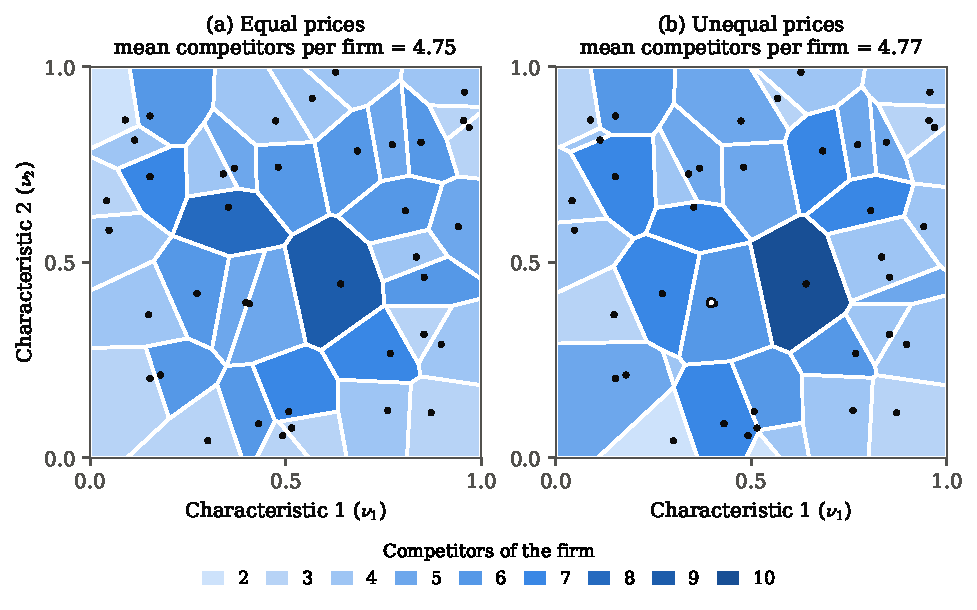
\includegraphics[width=\linewidth]{figures/ch04/voronoi.pdf}
\caption{Market areas of 40 products in a two-dimensional characteristics space. Consumers' ideal points are uniform
on the unit square, mismatch costs are quadratic, and dots mark product locations. Shading gives each firm's number
of competitors. (a) Equal prices: Voronoi cells. The average number of competitors is 4.75 over all 40 firms and
5.83 over the 18 firms whose areas do not touch the boundary. (b) Prices drawn between 1.000 and 1.012: power
diagram. One product (open circle) has no buyers. The average is 4.77 over the 39 active firms and 5.72 over the
18 interior firms. Computed with \texttt{figures/ch04/src/voronoi.py}.}
\label{fig:04-voronoi}
\end{figure}

The averages in the figure lie below six, as the proposition requires. Firms at the edge of the market have few
competitors, which pulls the overall average down. As the number of firms grows, the boundary matters less and
the average approaches six from below. Over random draws of uniform locations with equal prices, the average number
of competitors is 3.72 with 10 firms, 4.87 with 40, 5.43 with 160, 5.72 with 640 and 5.80 with 1,280. For firms
away from the boundary the averages are 5.16, 5.71, 5.87, 5.94 and 5.96.

\begin{remark}[Why competitors are defined by shared boundaries]\label{rem:04-competitor-def}
The definition of \citet{CaplinNalebuff1991} counts $k$ as a competitor of $j$ if a marginal cut in $p_j$
reduces $q_k$. Read as a nonzero derivative, it agrees with the shared-boundary definition when the type density
is positive on the interior of $B$. Read literally, as any loss of demand after a small cut, it counts
second-order losses too. Under the literal reading the bound in \cref{prop:04-cn-six} fails in degenerate
configurations. Place
$J \geq 8$ products at equal prices, equally spaced on a circle, with the quadratic mismatch costs of
\cref{fig:04-voronoi}. Let types be uniform on a disk with the same center. The Voronoi cells are wedges that
all meet at the center, and each shares edges only with its two neighbors. After a cut of size $\eta > 0$ in $p_j$, product $j$ is the strict favorite of every type near the
center, so it takes buyers from every other wedge. For a wedge that touches $j$'s area only at the center, the
lost area is of order $\eta^2$, and its first-order cross-price effect is zero. Under the literal reading every
firm has $J - 1 > 6$ competitors. Under the shared-boundary definition every firm has two, as the proposition
allows.
\end{remark}

\begin{example}[No bound in three dimensions]\label{ex:04-no-bound-3d}
Let $L = 3$ and let a consumer buy the product that minimizes $p_j + \tau\|\nu - x_j\|^2$, as in
\cref{fig:04-voronoi}. At equal prices the market areas are Voronoi cells. Types are uniform on the ball of
radius 2 around the origin, which satisfies A2.
Place $n$ products at $A_i = (a_i, 0, 0)$ and $n$ products at $B_l = (1, b_l, 1)$, with distinct $a_i \in [0, 1]$
and distinct $b_l \in [0, 1]$. The two groups lie on two skew lines. For each pair $(i, l)$ let
\begin{equation*}
z_{il} = \frac{(1 - a_i)^2 + 1 - b_l^2}{2}, \qquad c_{il} = (a_i, b_l, z_{il}).
\end{equation*}
The squared distances from $c_{il}$ to $A_i$ and to $B_l$ both equal $b_l^2 + z_{il}^2$. The squared distance to
any other $A_k$ is larger by $(a_k - a_i)^2 > 0$, and the squared distance to any other $B_k$ is larger by
$(b_k - b_l)^2 > 0$. By continuity, the types near $c_{il}$ on the plane of indifference between $A_i$ and $B_l$
are strictly closer to these two locations than to any other. Since $0 \leq z_{il} \leq 1$, the point $c_{il}$
lies inside the ball. The market areas of the two products therefore share a face of positive area within the
support. All $n^2$ such pairs are competitors under the sharper definition, and every product has positive
demand. With $J = 2n$ firms the average number of competitors is at least $\frac{2n^2}{2n} = n = \frac{J}{2}$,
which grows without bound.
\end{example}

The result matters for empirical work in two ways. A pure characteristics model in one or two dimensions implies a
sparse matrix of cross-price effects, in which a product's diversion goes on average to at most six neighbors. In
three or more dimensions the sparsity depends on the configuration of products (\cref{ex:04-no-bound-3d}). A logit-type model
spreads every product's diversion over all products. These are very different predictions for a merger between
two products, and the choice between them is made when the researcher picks the dimension of the model. The result
also shows that the location models of \cref{sec:04-location}, with one dimension, impose strong restrictions on
preferences, and that richer competition requires more dimensions.

\subsection{Demand systems in product space}\label{sec:04-spaces-product}

The goal of product-space demand analysis is to estimate $q = f(p, z)$ in a form that is flexible and consistent
with consumer theory. Aggregation is the main theoretical issue. Market demand behaves like the demand of a single
utility-maximizing consumer only under restrictions on individual preferences. Two such restrictions are the Gorman
polar form and the price-independent generalized logarithmic (PIGLOG) class (\cref{ch:aids}).
\Cref{tab:04-productspace-systems} summarizes the four classical systems. In the table and in this subsection goods are indexed by $i$ and $k$, as in \cref{ch:aids}. Total expenditure is $y$, and
$w_i = \frac{p_i q_i}{y}$ is the budget share of good $i$.

\begin{table}[htbp]
\centering
\caption{Classical demand systems in product space}
\label{tab:04-productspace-systems}
\footnotesize
\renewcommand{\arraystretch}{1.35}
\begin{tabularx}{\textwidth}{@{}>{\raggedright\arraybackslash}p{2.15cm}>{\raggedright\arraybackslash}p{4.35cm}%
>{\raggedright\arraybackslash}p{1.9cm}>{\raggedright\arraybackslash}p{2.7cm}>{\raggedright\arraybackslash}X@{}}
\toprule
System and source & Demand equation & Price parameters & Restrictions of theory & Main limitation \\
\midrule
Linear expenditure system \citep{Stone1954}
 & $p_iq_i = p_i\gamma_i + \beta_i\big(y - \sum_k p_k\gamma_k\big)$, from Stone-Geary utility $\sum_i\beta_i\ln(q_i -
   \gamma_i)$ with $\sum_i\beta_i = 1$
 & None beyond the $2J - 1$ parameters $(\gamma, \beta)$
 & Adding up, homogeneity and symmetry hold by construction
 & Too few parameters to be flexible. All goods are Hicksian substitutes, and no good is inferior. \\
Rotterdam model \citep{Theil1965,Barten1966}
 & $w_i\,\dd\ln q_i = \theta_i\,\dd\ln\bar Q + \sum_k\pi_{ik}\,\dd\ln p_k$, with $\dd\ln\bar Q = \sum_k w_k\,\dd\ln
   q_k$
 & $\frac{J(J-1)}{2}$ free $\pi_{ik}$
 & Adding up, homogeneity and symmetry are linear restrictions on $(\theta, \pi)$. Negativity needs $[\pi_{ik}]$
   negative semidefinite
 & A local approximation in differentials, with constant coefficients, not derived from a utility function. \\
Indirect translog \citep{ChristensenJorgensonLau1975}
 & $w_i = \frac{\alpha_i + \sum_k\beta_{ik}\ln\frac{p_k}{y}}{\sum_l\alpha_l + \sum_l\sum_k\beta_{lk}\ln\frac{p_k}{y}}$,
   by Roy's identity from a quadratic $\ln V$ in $\ln\frac{p}{y}$
 & $\frac{J(J+1)}{2}$ symmetric $\beta_{ik}$, less a normalization
 & Homogeneity and adding up built in. Symmetry imposed by $\beta_{ik} = \beta_{ki}$
 & Shares nonlinear in parameters. Aggregates only under extra restrictions. \\
Almost Ideal Demand System \citep{DeatonMuellbauer1980a}
 & $w_i = \alpha_i + \sum_k\gamma_{ik}\ln p_k + \beta_i\ln\frac{y}{P}$, with translog price index $\ln P$
 & $\frac{J(J-1)}{2}$ free $\gamma_{ik}$
 & Linear and testable: adding up, homogeneity, symmetry
 & Still of order $J^2$ parameters. Negativity not imposed globally. \\
\bottomrule
\end{tabularx}

\vspace{3pt}
\begin{minipage}{0.97\textwidth}
\footnotesize Notes: Goods are indexed by $i$ and $k$, $y$ is total expenditure and $w_i = \frac{p_iq_i}{y}$ is a
budget share. Parameter symbols are specific to each row. For the AIDS, $\ln P = \alpha_0 + \sum_k\alpha_k\ln p_k
+ \frac{1}{2}\sum_k\sum_l\gamma_{kl}\ln p_k\ln p_l$, and the restrictions are $\sum_i\alpha_i = 1$,
$\sum_i\gamma_{ik} = 0$, $\sum_i\beta_i = 0$ (adding up), $\sum_k\gamma_{ik} = 0$ (homogeneity) and $\gamma_{ik} =
\gamma_{ki}$ (symmetry) \citep[eqs.~8--12]{DeatonMuellbauer1980a}. In the Rotterdam model $\dd\ln\bar Q$ is the
Divisia volume index. Price-parameter counts are after the restrictions of theory.
\end{minipage}
\end{table}

The linear expenditure system was the first system estimated from an explicit utility function
\citep[p.~312]{DeatonMuellbauer1980a}. Consumers buy subsistence quantities $\gamma_i$ first and split the remaining
income in the fixed proportions $\beta_i$. Its cross-price effects are $\frac{\partial q_i}{\partial p_k} =
-\frac{\beta_i\gamma_k}{p_i}$ for $k \neq i$, so the $J^2$ price effects are pinned down by $2J - 1$ parameters. The
Rotterdam model approximates the demand functions themselves in differential form. The translog approximates the
indirect utility function to second order. The Almost Ideal Demand System starts from a class of preferences that
aggregates across consumers and yields shares that are nearly linear in the parameters. \Cref{ch:aids} develops the
AIDS in full, and \cref{rem:05-translog-piglog} states when the translog aggregates.

\casehead{Three problems in practice}
The first problem is dimensionality. A linear system $q = a + Ap$ has $J$ intercepts and $J^2$ price
coefficients. With $J = 50$ brands, as in a cereal aisle, that is 2,500 price coefficients. Symmetry reduces the
count to $\frac{J(J+1)}{2} = 1{,}275$, and the full set of AIDS restrictions to $\frac{J(J-1)}{2} = 1{,}225$. These
numbers exceed what typical market-level data can estimate.

The second problem is instruments. Each demand equation contains all $J$ prices, and every price is endogenous. Write
the equation for good $i$ in market $t$ as $q_{it} = a_i + \sum_k A_{ik}p_{kt} + e_{it}$, and let $z_t$ be a vector
of excluded instruments. The order condition requires at least $J$ instruments. The rank condition requires that
$\E[z_t p_t^\top]$ have rank $J$, so the instruments must move the $J$ prices independently of one another. A single
market-wide cost shifter fails this test. If $z_t$ is a scalar, the first-stage fitted prices $\hat p_{kt} =
\hat\pi_k z_t$ are proportional to one another, and only one linear combination of the row $A_{i\cdot}$ is
identified. Identification needs product-specific shifters, such as ingredient costs that differ across products,
or prices of the same product in other markets (\cref{ch:aids}).

The third problem is consumer heterogeneity. A representative consumer cannot say who gains and who loses from a
price change or a new product. Distributional questions, and substitution patterns that depend on who buys which
product, require explicit heterogeneity. Characteristics models build it in through the taste distribution and
demographics.

\casehead{Four ways forward}
Applied work responds to these problems in four ways. Each buys tractability with an assumption.
\begin{enumerate}
  \item \emph{Aggregate, or study one product.} Group products into a few aggregates, or estimate the residual
  demand of a single firm, as \citet{BakerBresnahan1988} do (\cref{ch:conduct}). This sacrifices the cross-effects
  among products within each aggregate.
  \item \emph{Impose symmetry.} Representative-consumer systems such as CES and logit treat products symmetrically
  up to one or two parameters (\cref{sec:04-repcons}). They suit questions about variety and poorly serve questions
  about which products are close substitutes.
  \item \emph{Impose separability.} Multi-stage budgeting splits goods into groups and estimates a small system within
  each group (\cref{sec:05-separability}). \citet{HausmanLeonardZona1994} and \citet{Hausman1997} follow this route
  with the AIDS at the lowest level.
  \item \emph{Move to characteristics space.} Discrete choice models replace product-indexed parameters with tastes for
  characteristics (\cref{ch:discrete,ch:logit,ch:blp}), at the costs described in \cref{sec:04-spaces-drawbacks}.
\end{enumerate}
The rest of this chapter develops the second route, together with the location models that underlie the fourth.
\Cref{ch:aids} takes the third route, and \cref{ch:discrete,ch:logit,ch:blp} take the fourth.
